% Options for packages loaded elsewhere
\PassOptionsToPackage{unicode}{hyperref}
\PassOptionsToPackage{hyphens}{url}
\PassOptionsToPackage{dvipsnames,svgnames,x11names}{xcolor}
%
\documentclass[
  11pt,
  letterpaper]{article}
\usepackage{amsmath,amssymb}
\usepackage{iftex}
\ifPDFTeX
  \usepackage[T1]{fontenc}
  \usepackage[utf8]{inputenc}
  \usepackage{textcomp} % provide euro and other symbols
\else % if luatex or xetex
  \usepackage{unicode-math} % this also loads fontspec
  \defaultfontfeatures{Scale=MatchLowercase}
  \defaultfontfeatures[\rmfamily]{Ligatures=TeX,Scale=1}
\fi
\usepackage{lmodern}
\ifPDFTeX\else
  % xetex/luatex font selection
\fi
% Use upquote if available, for straight quotes in verbatim environments
\IfFileExists{upquote.sty}{\usepackage{upquote}}{}
\IfFileExists{microtype.sty}{% use microtype if available
  \usepackage[]{microtype}
  \UseMicrotypeSet[protrusion]{basicmath} % disable protrusion for tt fonts
}{}
\makeatletter
\@ifundefined{KOMAClassName}{% if non-KOMA class
  \IfFileExists{parskip.sty}{%
    \usepackage{parskip}
  }{% else
    \setlength{\parindent}{0pt}
    \setlength{\parskip}{6pt plus 2pt minus 1pt}}
}{% if KOMA class
  \KOMAoptions{parskip=half}}
\makeatother
\usepackage{xcolor}
\usepackage[margin=1in]{geometry}
\usepackage{color}
\usepackage{fancyvrb}
\newcommand{\VerbBar}{|}
\newcommand{\VERB}{\Verb[commandchars=\\\{\}]}
\DefineVerbatimEnvironment{Highlighting}{Verbatim}{commandchars=\\\{\}}
% Add ',fontsize=\small' for more characters per line
\usepackage{framed}
\definecolor{shadecolor}{RGB}{248,248,248}
\newenvironment{Shaded}{\begin{snugshade}}{\end{snugshade}}
\newcommand{\AlertTok}[1]{\textcolor[rgb]{0.94,0.16,0.16}{#1}}
\newcommand{\AnnotationTok}[1]{\textcolor[rgb]{0.56,0.35,0.01}{\textbf{\textit{#1}}}}
\newcommand{\AttributeTok}[1]{\textcolor[rgb]{0.13,0.29,0.53}{#1}}
\newcommand{\BaseNTok}[1]{\textcolor[rgb]{0.00,0.00,0.81}{#1}}
\newcommand{\BuiltInTok}[1]{#1}
\newcommand{\CharTok}[1]{\textcolor[rgb]{0.31,0.60,0.02}{#1}}
\newcommand{\CommentTok}[1]{\textcolor[rgb]{0.56,0.35,0.01}{\textit{#1}}}
\newcommand{\CommentVarTok}[1]{\textcolor[rgb]{0.56,0.35,0.01}{\textbf{\textit{#1}}}}
\newcommand{\ConstantTok}[1]{\textcolor[rgb]{0.56,0.35,0.01}{#1}}
\newcommand{\ControlFlowTok}[1]{\textcolor[rgb]{0.13,0.29,0.53}{\textbf{#1}}}
\newcommand{\DataTypeTok}[1]{\textcolor[rgb]{0.13,0.29,0.53}{#1}}
\newcommand{\DecValTok}[1]{\textcolor[rgb]{0.00,0.00,0.81}{#1}}
\newcommand{\DocumentationTok}[1]{\textcolor[rgb]{0.56,0.35,0.01}{\textbf{\textit{#1}}}}
\newcommand{\ErrorTok}[1]{\textcolor[rgb]{0.64,0.00,0.00}{\textbf{#1}}}
\newcommand{\ExtensionTok}[1]{#1}
\newcommand{\FloatTok}[1]{\textcolor[rgb]{0.00,0.00,0.81}{#1}}
\newcommand{\FunctionTok}[1]{\textcolor[rgb]{0.13,0.29,0.53}{\textbf{#1}}}
\newcommand{\ImportTok}[1]{#1}
\newcommand{\InformationTok}[1]{\textcolor[rgb]{0.56,0.35,0.01}{\textbf{\textit{#1}}}}
\newcommand{\KeywordTok}[1]{\textcolor[rgb]{0.13,0.29,0.53}{\textbf{#1}}}
\newcommand{\NormalTok}[1]{#1}
\newcommand{\OperatorTok}[1]{\textcolor[rgb]{0.81,0.36,0.00}{\textbf{#1}}}
\newcommand{\OtherTok}[1]{\textcolor[rgb]{0.56,0.35,0.01}{#1}}
\newcommand{\PreprocessorTok}[1]{\textcolor[rgb]{0.56,0.35,0.01}{\textit{#1}}}
\newcommand{\RegionMarkerTok}[1]{#1}
\newcommand{\SpecialCharTok}[1]{\textcolor[rgb]{0.81,0.36,0.00}{\textbf{#1}}}
\newcommand{\SpecialStringTok}[1]{\textcolor[rgb]{0.31,0.60,0.02}{#1}}
\newcommand{\StringTok}[1]{\textcolor[rgb]{0.31,0.60,0.02}{#1}}
\newcommand{\VariableTok}[1]{\textcolor[rgb]{0.00,0.00,0.00}{#1}}
\newcommand{\VerbatimStringTok}[1]{\textcolor[rgb]{0.31,0.60,0.02}{#1}}
\newcommand{\WarningTok}[1]{\textcolor[rgb]{0.56,0.35,0.01}{\textbf{\textit{#1}}}}
\usepackage{graphicx}
\makeatletter
\newsavebox\pandoc@box
\newcommand*\pandocbounded[1]{% scales image to fit in text height/width
  \sbox\pandoc@box{#1}%
  \Gscale@div\@tempa{\textheight}{\dimexpr\ht\pandoc@box+\dp\pandoc@box\relax}%
  \Gscale@div\@tempb{\linewidth}{\wd\pandoc@box}%
  \ifdim\@tempb\p@<\@tempa\p@\let\@tempa\@tempb\fi% select the smaller of both
  \ifdim\@tempa\p@<\p@\scalebox{\@tempa}{\usebox\pandoc@box}%
  \else\usebox{\pandoc@box}%
  \fi%
}
% Set default figure placement to htbp
\def\fps@figure{htbp}
\makeatother
\setlength{\emergencystretch}{3em} % prevent overfull lines
\providecommand{\tightlist}{%
  \setlength{\itemsep}{0pt}\setlength{\parskip}{0pt}}
\setcounter{secnumdepth}{-\maxdimen} % remove section numbering
\usepackage[notextcomp]{kpfonts}
\usepackage{Inconsolata}
\usepackage{caption}
\usepackage{float}
\captionsetup*{labelfont={sc},textfont={it},labelsep={colon},justification=centering,singlelinecheck=true}
\usepackage{bookmark}
\IfFileExists{xurl.sty}{\usepackage{xurl}}{} % add URL line breaks if available
\urlstyle{same}
\hypersetup{
  pdfauthor={John Koo},
  pdfsubject={Week 1 Handout},
  colorlinks=true,
  linkcolor={Maroon},
  filecolor={Maroon},
  citecolor={Blue},
  urlcolor={blue},
  pdfcreator={LaTeX via pandoc}}

\title{\textsc{Week 1 Handout}}
\usepackage{etoolbox}
\makeatletter
\providecommand{\subtitle}[1]{% add subtitle to \maketitle
  \apptocmd{\@title}{\par {\large #1 \par}}{}{}
}
\makeatother
\subtitle{Gov 50 Data Science for the Social Sciences}
\author{John Koo}
\date{September 2, 2025}

\begin{document}
\maketitle

\section{Contact Info}\label{contact-info}

\begin{table}[!h]

\centering

\begin{tabular}{l}
  \textbf{John Koo} \\
  PhD Candidate, Department of Government \\ \\
  
  \textbf{Email} (preferred): \href{mailto:johnkoo@fas.harvard.edu}{johnkoo@fas.harvard.edu} \\
  \textbf{Slack}: @johnkoo (in the Harvard University workspace) \\
  \textbf{Office hours}: Tuesdays, 1:30pm to 3:30pm @ CGIS Caf\'e (sign-up: \href{https://jkoo.nl/meet}{jkoo.nl/meet}) \\ \\ 
  \textbf{Section materials}: \url{https://github.com/tanxpyox/gov50-sections-jk}
  
  \end{tabular}
\end{table}

\section{Where to get help?}\label{where-to-get-help}

\begin{itemize}
\item
  For tech assistance or help with homework: \textbf{Course
  Assistant-led Study Halls}

  \begin{quote}
  Study halls are a combination of office hours and drop-in tutoring
  sessions. Course assistants will hold a table usually at the CGIS
  Fisher Family Commons and help students with assignments and course
  material. Study halls work best if you come as a group and work on the
  assignments on your own while you are there and ask for help from the
  CAs when you get stuck.
  \end{quote}

  \begin{quote}
  Schedule: Mondays and Wednesdays, 5pm to 9pm (see Syllabus for
  location)
  \end{quote}
\item
  For help with course content: ask on course Slack (accessible via
  Canvas sidebar) or sign up for my office hours
\item
  For perspective and inspiration: sign up for Scott's office hours:
  \url{https://calendly.com/causalinf/office-hours}
\end{itemize}

\section{Getting the most (grades) out of this
class}\label{getting-the-most-grades-out-of-this-class}

\begin{itemize}
\tightlist
\item
  Podcast and Article Responses (5\%) {[}one two-page doc every other
  week{]}
\item
  Problem Sets (20\%) {[}seven to eight in total{]}
\item
  Mid-term exam (20\%) {[}in-class, written, closed book{]}
\item
  Final exam (20\%) {[}in-class, written, closed book{]}
\item
  \emph{Final project} (25\%)
\end{itemize}

\newpage

Generic advice for maximising grades and efficiency

\begin{itemize}
\tightlist
\item
  Everything you learn should help you work towards the final project
  (which is the biggest chunk of your grades)

  \begin{itemize}
  \tightlist
  \item
    Take the project milestones seriously and do not wait until the last
    minute
  \end{itemize}
\item
  Problem sets

  \begin{itemize}
  \tightlist
  \item
    Low hanging fruit - don't miss them; Can reuse code in your projects
  \item
    It's OK to make mistakes (each p-set is 2--3\% of your final grade)
  \item
    Work with your study group; but write up your p-sets individually
  \item
    Start early, so you have time to get help
  \item
    Set aside a ``focus session'' every week to do the problem sets; do
    not mull over the p-set for the whole week
  \end{itemize}
\item
  AI allowed, except in exams. Start learning how to use AI to debug
  your code.
\item
  Keep your code organised in your GitHub repository - you may need them
  in your final project
\end{itemize}

\section{Getting Started}\label{getting-started}

\begin{itemize}
\item
  Software: R, RStudio
\item
  Version control: Git and GitHub
\end{itemize}

\begin{figure}
\centering
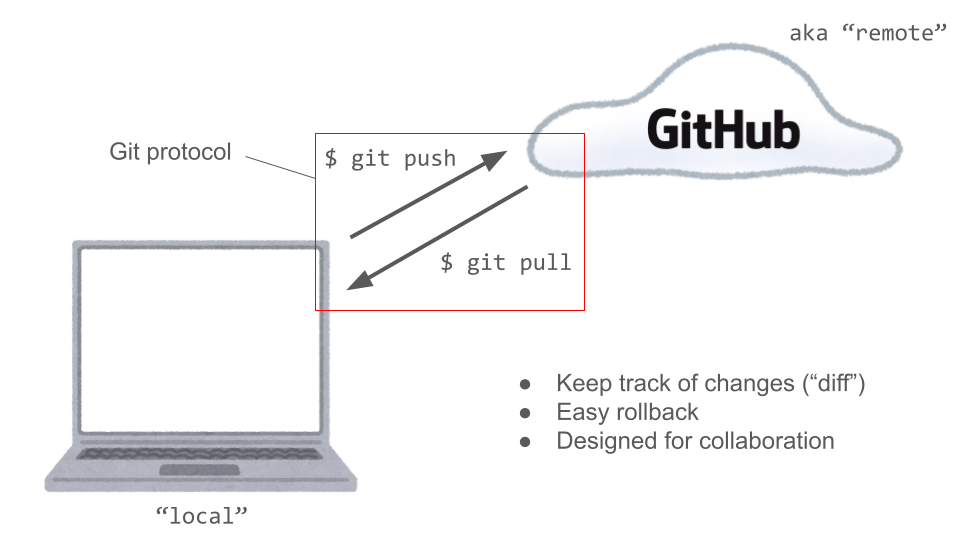
\includegraphics[width=0.75\linewidth,height=\textheight,keepaspectratio]{assets/gitvsgithub.png}
\caption{Git and GitHub}
\end{figure}

\newpage

\begin{center}
  \section{Problem Set 0: Getting Started with R, R Studio, and Slack}
  \textbf{Due: Wednesday, September 10, 2025 at 11:59 PM}
\end{center}

\subsection{Installing R and RStudio}\label{installing-r-and-rstudio}

In this problem set, we're going to get R, RStudio, and R Markdown set
up on your computer. To get started, follow these steps:

\begin{enumerate}
\def\labelenumi{\arabic{enumi}.}
\item
  Download and install the most recent version of
  \href{https://cloud.r-project.org/}{R (click me)}. There are versions
  available for the Windows, Mac, and Linux operating systems. On a
  Windows machine, you will want to install using the
  \texttt{R-x.y.z-win.exe} file where \texttt{x.y.z} is a version
  number. On a Mac, you will want to install using the
  \texttt{R-x.y.z.pkg} file that is notarized and signed.
\item
  With R installed, download and install
  \href{https://posit.co/download/rstudio-desktop/}{RStudio (click me)}.
  RStudio is a type of ``integrated development environment'' or IDE
  designed for R. It makes working with R considerably easier and is
  available for most platforms. It is also free.
\item
  Open the .Rmd version of this file in RStudio. Install the packages we
  will use throughout the semester. To do this, either type or copy and
  paste each of the following lines of code into the ``Console'' in
  RStudio (lower left panel by default). Make sure you do this
  separately for each line. If you are asked if you want to install any
  packages from source, type ``no''. Note that the symbols next to
  \texttt{my\_package} are a less than sign \texttt{\textless{}}
  followed by a minus sign \texttt{-} with no space between them. (Don't
  be worried if you see some red text here. Those are usually just
  messages telling you information about the packages you are
  installing. Unless you see the word \texttt{Error} you should be
  fine.)
\end{enumerate}

\begin{Shaded}
\begin{Highlighting}[]
\NormalTok{my\_packages }\OtherTok{\textless{}{-}} \FunctionTok{c}\NormalTok{(}\StringTok{"tidyverse"}\NormalTok{, }\StringTok{"usethis"}\NormalTok{, }\StringTok{"devtools"}\NormalTok{, }\StringTok{"learnr"}\NormalTok{,}
                 \StringTok{"gitcreds"}\NormalTok{)}
\FunctionTok{install.packages}\NormalTok{(my\_packages, }\AttributeTok{repos =} \StringTok{"http://cran.rstudio.com"}\NormalTok{)}
\end{Highlighting}
\end{Shaded}

\begin{enumerate}
\def\labelenumi{\arabic{enumi}.}
\setcounter{enumi}{3}
\tightlist
\item
  For some things in the course, we'll need produce PDFs from R and that
  requires something called LaTeX. If you've never heard of that, it's
  completely fine and you should just run the following two lines of R
  code:
\end{enumerate}

\begin{Shaded}
\begin{Highlighting}[]
\FunctionTok{install.packages}\NormalTok{(}\StringTok{\textquotesingle{}tinytex\textquotesingle{}}\NormalTok{)}
\NormalTok{tinytex}\SpecialCharTok{::}\FunctionTok{install\_tinytex}\NormalTok{()  }\CommentTok{\# install TinyTeX}
\end{Highlighting}
\end{Shaded}

\subsection{Joining the Course Slack}\label{joining-the-course-slack}

\begin{enumerate}
\def\labelenumi{\arabic{enumi}.}
\setcounter{enumi}{4}
\tightlist
\item
  In the left hand menu on Canvas click the item called Slack. Slack is
  the main way forum we will use to send out announcements and answer
  questions for this course. Post a short introduction message in the
  \#general channel
  (e.g.~\texttt{Hi\ all,\ my\ name\ is\ Noah\ and\ I\textquotesingle{}m\ looking\ forward\ to\ this\ class})
\end{enumerate}

\subsection{Submitting}\label{submitting}

\begin{enumerate}
\def\labelenumi{\arabic{enumi}.}
\setcounter{enumi}{5}
\tightlist
\item
  Click the \texttt{Knit} button near the top of the RStudio window,
  this should create a pdf version of this document in the same place
  you are storing this .Rmd file (we strongly recommend having a
  dedicated folder for Gov50 assignments). If you encounter any issues
  knitting seek help from a TF or CA. Upload the pdf in Gradescope (can
  be reached via the left hand menu on Canvas) under the assignment
  \texttt{Problem\ Set\ 0:\ Getting\ Started}. This along with your
  written introduction in Slack constitutes the assignment. This
  assignment is graded on completion only.
\end{enumerate}

\end{document}
